\documentclass{UoYCSproject}
\usepackage{color,soul}
\usepackage{graphicx}
\usepackage{amsmath}
\usepackage{textgreek}
\usepackage{amssymb}

\addbibresource{refs.bib}

\author{Patrick Buhagiar}
\title{The Impact of Macroeconomic Parameters on Forecasting Financial Markets}
\date{2018-July-30}
\supervisor{Dimitar Kazakov}
\MIP
\wordcount{3884}

\includes{Appendices \ref{cha:usefulpackages}, \ref{cha:gotchas} and
  \ref{cha:deptfac}}

\excludes{\autoref{cha:quoteex}}

\abstract{ 
    Financial forecasting is a common area in machine learning, however a gap in literature was identified with respect to the influence of macroeconomic variables in predicting financial markets. This study attempts to use ensemble methods to predict the direction of the FTSE market in relation to other financial markets and macroeconomic variables in the UK. This study adopts a two-stage process. The first stage consists of creating several ANN models for different time periods that predict the stock market based on the closing prices of other markets. The second stage consists of feeding the results from the first stage and macroeconomic data into another ANN. \hl{TODO add result summary as last sentence}
}

\dedication{To all students everywhere}

\acknowledgements{To my cactus, that I forget to water}
\bibliography{refs}
\begin{document}

\maketitle

\listoffigures
\listoftables

\label{sec:start}
\thispagestyle{empty}\cleardoublepage

\chapter{Introduction}
\label{cha:Introduction}

\chapter{Literature Review}
\label{cha:literaturereview}

\section{Macro and Micro Economics}
\label{macroandmicro}
According to Adam Smith, the first modern economist, the economy is a mix of micro and macroeconomics where every entity has individual interest towards gain, such that this gain is also linked to the overall benefit of the market as a whole \cite{smith1950inquiry}. Macroeconomics is the study of the behaviour, performance and trends of an economy as a whole. Macro-economists evaluate a variety of economy-wide phenomena such as inflation, gross domestic product (GDP) and unemployment. To keep the economy in check, governments look at these factors to aid in economic policy decision making. Microeconomics on the other hand is the study of how individuals make economic decisions and their effect on the economy. These individuals are classified into consumers, producers and resource owners \cite{dwivedi2002microeconomics}. These individuals interact with the supply and demand for resources while using indications such as interest rates and money as a pricing mechanism for coordination. 

Despite being split into two different studies, macroeconomics and microeconomics are deeply interlinked with each other since they contain overlapping issues. They can be considered as opposite approaches, where macroeconomics take a top-down approach and microeconomics a bottom-up approach to analysing an economy. As an example of how these two studies complement each other, it is evident that a stock market's long-run performance is heavily coupled with the economy's performance \cite{davis2008macroeconomic}. This coupled relationship can be seen in Figure \ref{fig:gdpvssp500} which shows a normalised plot for the U.S. GDP and the S\&P 500 index. In this case, it comes to no surprise that investment analysts focus on economic performance expectations to determine the future prospects of stock markets.

\begin{figure}[h]
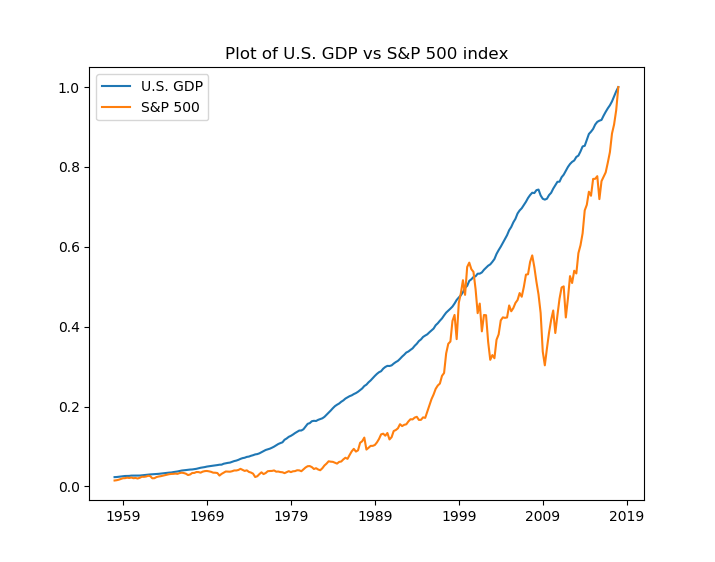
\includegraphics[width=10cm]{GDPvsSP500}
\centering
\caption{Normalised quarterly data from 1958 to 2018 for U.S. GDP and S\&P 500 index. Sources: Standard \& Poor's, U.S. Census Bureau} 
\label{fig:gdpvssp500}
\end{figure}

\subsection{Inflation}
Inflation is the rate at which the general level of prices for goods and services is rising \cite{inflation}. As a result of inflation, the purchasing power of a currency decreases. If the price of milk costs \pounds 1 this year, then with an inflation rate of 2\% it will cost \pounds 1.02 the following year. Deflation is the opposite of inflation, where the general level of prices decreases. Central banks define this inflation rate and try to limit inflation, while avoiding deflation, so as to keep the economy running smoothly. While over inflation should be avoided, deflation is much more catastrophic and has helped cause the worst economic meltdowns in U.S. history \cite{fleckenstein2013deflation}. If there is deflation, people refrain from consuming goods because they know that prices will be cheaper in the future. This will reduce the demand for goods drastically which will cut corporate profits, lower wages and reduce the work force, hence resulting in a weaker economy. For an economy to function well, both the consumers and producers must be willing to consume and produce. 

\subsection{Balance of Trade}
The balance of trade is the difference between the value of a country's imports and exports during a certain period \cite{balanceoftrade}. Economists refer to the balance of trade to measure the relative strength of a country's economy. The balance of trade can be calculated with the following simple formula:

\begin{equation}
    Balance Of Trade = Imports - Exports
\end{equation}

When a country imports more than it exports, it would have a trade deficit, otherwise if it exports more than it imports it would have a trade surplus. A country that has a trade deficit borrows money. This could lead to the value of the country's currency to fall, which will result in consumers paying more for foreign imports \cite{2003economics}. Alternatively, a country that has a trade surplus lends money to deficit countries. As of 2016, the country with the highest trade surplus is China, with a surplus of \$510 Billion \cite{tradesurplus}.   

\subsection{GDP}
Historically, the gross domestic product (GDP) is one of the most important variables when it comes to measuring the health of an economy. A country's GDP is the total value of all final goods and services produced in the economy \cite{2003economics}. GDP helps define the size of an economy. The bigger the GDP, the more goods are being produced, therefore the healthier the economy.  There are many factors that effect the GDP such as life expectancy, higher initial schooling, lower inflation and lower fertility \cite{barro1996determinants}. 

\subsection{Unemployment Rate}
The unemployment rate is the percentage of the labour force that is jobless \cite{unemployment}. In a weak economy, jobs tend to be scarce, hence the unemployment rate is expected to rise. Alternatively, a healthy economy is more likely to have more jobs available, thus the unemployment rate will decrease. This means that unemployment rate is another factor that highly affects a country's GDP \cite{bean1993unemployment}. A low unemployment rate means that more people are employed and getting paid, which brings in more money into the economy, ergo increase GDP.  

\subsection{Interest Rate}
An interest rate is a percentage of the amount that one pays when borrowing or gets paid when saving money \cite{interestrate}. If \pounds 1000 is placed into a savings account with a 1\% interest rate, there will be \pounds 1010 the following year.  The bank rate is the most important interest rate in an economy and is set by the central bank. The bank rate is the rate of interest payed on reserve balances held by commercial banks. Increasing the bank rate makes borrowing more expensive which means people will spend less in order to pay off their debts or benefit more from saving. In this scenario, inflation will decrease. Ultimately, interest rates can be considered as a tool for monetary policy that can be used to contain inflation within an expected range \cite{christiano1999monetary}. 

\section{Financial Markets}
\label{financialmarkets}
A financial market is a marketplace for buying and selling securities such as stocks, bonds and currencies \cite{financialmarket}. Trading occurs on what is called an exchange. In the case of stocks, this is called a stock exchange and can either be in a physical location (like NYSE) or an electronic system (like NASDAQ). Any company that is traded on an exchange is referred to as a listed company, otherwise securities that are not listed are sold Over-The-Counter (OTC). Companies that trade shares OTC are typically smaller and riskier companies that did not meet the requirements to be listed on the stock exchange \cite{stockexchange}. As of June 2017, the stock exchange with the highest market capitalisation is the New York Stock Exchange (NYSE) at \$21 trillion \cite{nyse}. 
These stock exchanges do not operate 24 hours a day and are closed throughout the weekend and bank holidays. Table \ref{tab:markets} lists the opening and closing times of some stock exchanges around the world. 

\begin{table}[h]
    \centering
    \begin{tabular}{|c|c|c|} \hline
        \textbf{Stock Exchange} & \textbf{Open (UTC)} & \textbf{Close (UTC)} \\ \hline
        London & 08:00 & 16:30 \\
        New York & 14:30 & 21:00 \\
        Paris & 08:00 & 16:30 \\
        Frankfurt & 07:00 & 19:00 \\
        Hong Kong & 01:30 & 08:00 \\
        Tokyo & 00:00 & 06:00 \\
        \hline
    \end{tabular}
    \caption{Opening and closing times of stock exchanges.}
    \label{tab:markets}
\end{table}

\subsection{Stock Market Index}
Another way to measure the value of a stock market, other than the total market capitalisation, is to refer to what is called a stock market index. A stock market index is computed from the prices or market capitalisation of a few selected stocks, typically from the largest and most influential companies in that market. The Dow Jones Industrial Average (DJIA) is one of the oldest, most well-known stock market index in the world, which takes the stocks prices of 30 companies in the United States across different industries, such as Apple, American Express, Coca-Cola and ExxonMobil. Experts however feel that the DJIA is \textit{"no longer a great reflection of the market anymore [since] it only covers 30 stocks [and] puts too much emphasis on the price rather than a market's capitalisation"} \cite{dowproblem}. For the United States, a better alternative is the S\&P 500, which is much more diverse than DJIA because it includes 500 companies and uses a market capitalisation-weighted index. The main goal of these stock market indices is to represent a broad economy. Table \ref{tab:indices} lists a few of the most common stock indices, along with the region and the number of companies they represent. 

\begin{table}[h]
    \centering
    \begin{tabular}{|c|c|c|c|} \hline
        \textbf{Index} & \textbf{Trading Symbol} & \textbf{Region} & \textbf{Index Size} \\ \hline
        DOW 30 & DJI & U.S.A & 30 \\
        S\&P 500 & GSPC & U.S.A & 500 \\
        NASDAQ 100 & NDX & U.S.A & 100 \\
        FTSE 100 & UKX & U.K. & 100 \\
        DAX & GDAXI & Germany & 30 \\
        CAC 40 & FCHI & France & 40 \\
        EURO STOXX 50 & SX5E & Eurozone & 50 \\
        NIKKEI 225 & NI225 & Japan & 225 \\
        HANG SENG & HSI & Hong Kong & 50 \\
        \hline
    \end{tabular}
    \caption{Table of Popular Stock Market Indices}
    \label{tab:indices}
\end{table}

\subsection{Market Contagion}
One of the major shifts in the last few decades is globalisation, which consequently has increased openness and interpenetration of national economies and sovereign states \cite{scott1999regions}. As a result, regional markets have started to be more correlated with each other. Market contagion refers to this correlation, where market changes or disturbances spread from one regional market to another. This means that a financial crisis in one region will create a domino effect and weaken other economies. A good example of this is the \textit{Great Depression} in the 1930s, which originated in the United States, and resulted in the global GDP falling by 15\% in the first 3 years \cite{rogerhistoryrepeating}.   

Market contagion can easily be visualised and quantified. Figure \ref{fig:stockindexplot} contains a scaled plot of the indices in Table \ref{tab:indices} over a 5 year period. From observing the structure of the indices, it is evident that markets are connected globally, where markets seem to fall and rise together. The scatter matrix plot in Figure \ref{fig:scatterplot} further emphasis the correlation between global markets. As this work will be predicting the direction of the FTSE index, we can see that FTSE has a strong correlation with CAC, DAX and STOXX, all of which are European markets. There is also good correlation with the S\&P 500, and less correlation with HKSE and NIKKEI. Table \ref{tab:correlations} quantifies the correlations between the FTSE stock market index and the other stock market indices mentioned in Table \ref{tab:indices}. 

\begin{figure}[h]
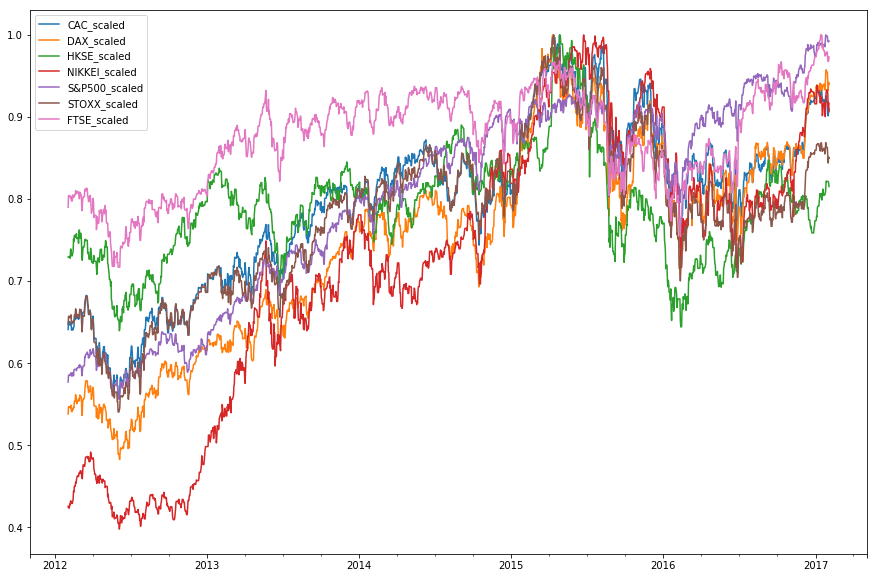
\includegraphics[width=12cm]{scaled_plot_of_indices}
\centering
\caption{A scaled plot of the CAC, DAX, HKSE, NIKKEI, S\&P 500, STOXX and FTSE stock market Indices} 
\label{fig:stockindexplot}
\end{figure}


\begin{figure}[h]
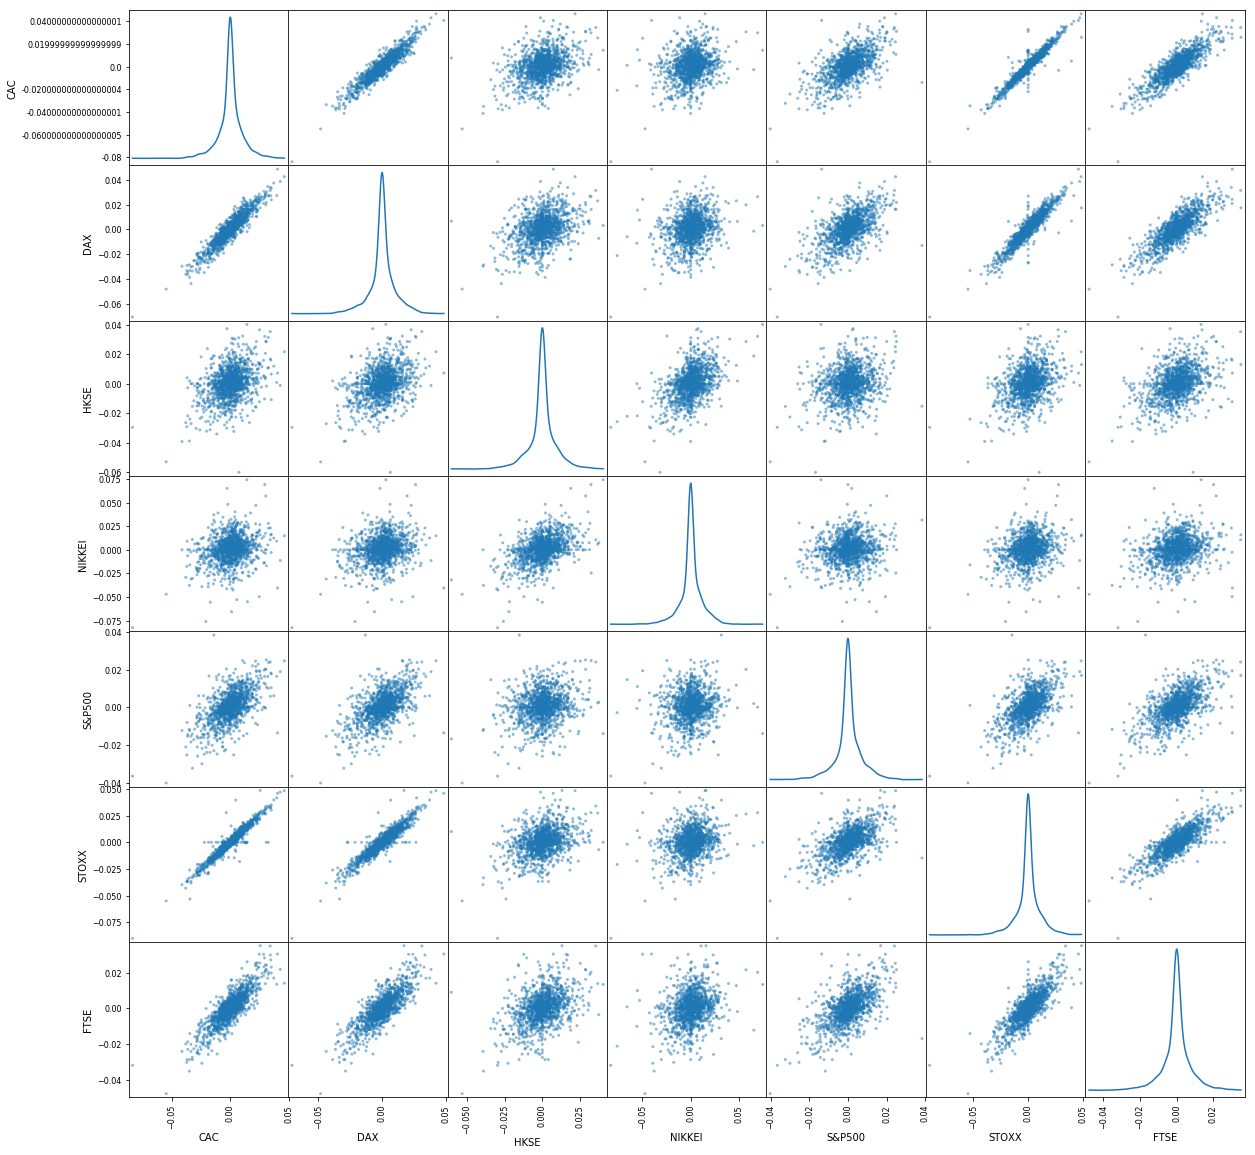
\includegraphics[width=12cm]{market_correlation}
\centering
\caption{A scatter matrix plot showing the correlations between each market.} 
\label{fig:scatterplot}
\end{figure}

\begin{table}[h]
    \centering
    \begin{tabular}{|c|c|} \hline
        \textbf{Stock Matket Index} & \textbf{Correlation} \\ \hline
        CAC &       0.848935 \\
        DAX  &     0.817487\\
        STOXX &    0.818773\\
        HKSE   &   0.417783\\
        NIKKEI  &  0.268837\\
        S\&P 500   & 0.587923\\

        \hline
    \end{tabular}
    \caption{The correlation between the FTSE stock market index and other stock market indices.}
    \label{tab:correlations}
\end{table}


\subsection{Market Hypotheses}
The following subsections will give a quick overview for some of the well known market hypotheses. A more detailed discussion can be found in Matthew Butler's work \cite{butler2012computational}.
\subsubsection{Efficient Market Hypothesis}
The Efficient Market Hypothesis (EMH) was introduced by Fama in 1970  \cite{malkiel1970efficient} and is frequently cited in the field of finance and economics as it is a ubiquitous theory in modern finance. It states that a market is said to be efficient if the stock price of a company, at any given time, truly reflects the value of that company. This means that there is no point in studying past stock prices in search for patterns to predict future prices. While many academics refer to a large body of evidence in support of EMH, an equal amount of evidence also contradicts EMH. Jensen's \cite{jensen1978some} paper finds that as better data is becoming available, such as daily stock prices, the more inconsistencies are beginning to be found with EMH. It concludes that there are flaws with EMH and over time we will better understand these flaws and thus a better understanding of the markets. Another paper by Malkiel \cite{malkiel2003efficient} points out that while evidence has proved EMH to be useful in the past, certain conditions have deemed EMH inefficient for the current modern economy. Nonetheless, economists have not yet reached a consensus about whether financial markets are indeed efficient \cite{lo2004adaptive}.  

\subsubsection{Adaptive Market Hypothesis}
AMH is an improved version of EMH by Andrew Lo \cite{lo2004adaptive}. He explains that emerging study has challenged EMH, arguing that markets are actually driven by fear and greed rather than being rational. AMH seeks to add behavioural alternatives to EMH by applying the principles of evolution to financial interactions where the market is seen as an evolving entity \cite{lo2004adaptive}. These evolutionary principles are competition, adaptation and natural selection. Lo further expands on AMH in another paper \cite{lo2005reconciling}
by delving into a neuroscience perspective.

\subsubsection{Random Walk Hypothesis}
The random walk hypothesis is another financial theory that is consistent with EMH. It states that stock prices are random, and thus cannot be predicted. It was introduced in Burton Malkiel's book "\textit{A Random Walk Down Wall Street}" \cite{malkiel1973random}. Similar to EMH, it also suggests that there is no point in exploiting patterns in historical data to gain profits.  

\subsubsection{Chaos Theory}
Chaos theory is a mathematical concept that deals with nonlinear models, therefore anything that is effectively impossible to predict or control, such as weather, brain states or, in this case, stock markets. In chaos theory, price changes can be determined through mathematical equations predicting factors such as a trader's own personal motives, volume changes, acceleration of the changes, and the momentum behind the changes \cite{chaostheory}. Chaos theory however is highly dependent on the initial conditions set, and produce very diverging outputs with the slightest change in inputs \cite{kellert1993wake}. 

\section{Analysis Techniques}
\subsection{Technical Analysis}
Technical analysis assumes that history tends to repeat itself, thus analysing past patterns can be used for predictive purposes \cite{levy1966conceptual}. For financial markets, this means looking at past stock prices for predictions rather than its components. There are three major assumptions:
\begin{enumerate}
    \item The stock price is reflective of the entire company's influential factors.
    \item Stock price movements follow trends.
    \item History repeats itself in terms of price movements.
\end{enumerate}

\subsection{Fundamental Analysis}
Fundamental analysis takes a wider approach than technical analysis by studying the past and present market data, as well as economic-level, industry-level and company-level indicators such as earnings, risk, growth and competitive position. Papers such as that of Lev and Thiagarajan \cite{lev1993fundamental} attempt to identify which fundamentals or financial variables, over a certain period of time, where suitable for performing financial forecasting. These fundamentals can either be quantitative or qualitative. Quantitative fundamentals are numeric values such as revenue and profit, while qualitative fundamentals are those that are based on the character or quality of a variable, such as brand recognition and competitive position. 

Unlike technical analysis, fundamental analysis assumes that the stock market is not fully representative of the actual value of the stock. fundamentalists however do believe that the market will reflect these fundamentals in the long run, thus encouraging investors to find opportunities to buy stocks at a reduced price by estimating the actual value of the stock. 

\subsection{Time series Analysis}
A time series is a collection of numerical data points collected at constant time in a form of a sequence. With time series analysis, we can obtain meaningful statistics and other characteristics of data, thus we can understand the data and build a model based on the given pattern. Extracting such models will allow us to forecast future values. 

Two key properties about time series are that they are time dependent, and that most time series have some form of seasonality trends. Seasonality trends mean that the time series consists of variations specific to a particular time frame. Due to these properties, forecasting time series requires the data to be stationary. A time series is said to be stationary if both the mean and autocovariances do not depend on the date \cite{hamilton1994time}. 

\subsubsection{Making a Series Stationary}
\label{subsec:stationary}
Making a time series stationary involves removing trends and seasonal changes. There are several methods for making a time series stationary, some of which can be combined together:
\begin{enumerate}
    \item \textbf{Transformation:} Trend can be reduced by transforming the data. this can be anything from calculating the log, square-root, cube root etc.  
    \item \textbf{Moving Average:} This method takes the average of \textit{k} consecutive values, depending on the frequency of the time series, for example 12 months, or 1 year. This is also called a \textit{rolling mean}. 
    \item \textbf{Differencing:} This technique involves subtracting each value with it's previous value.
    \item \textbf{Decomposition:} This approach consists of modelling trend and seasonality separately, and returning the remaining part, typically referred to as \textit{residual}. 
\end{enumerate}

\subsubsection{How to Test for Stationarity}
Statistical tests can be utilised to examine the stationary assumptions by decomposing the time series into three elements: trend, random walk, and stationary error. Two popular tests are the Kwiatkowski-Phillips-Schmidt-Shin (KPSS) test and the Augmented Dickey-Fuller (ADF) test.

The ADF test was introduced in 1979 by David Dickey and Wayne Filler \cite{dickey1979distribution}. This test is used to determine whether a unit root, a stochastic feature that can cause problems in statistical inference, is present in an autoregressive model. 

The KPSS method proposes a test of the null hypothesis that a series is stationary around a deterministic trend \cite{kwiatkowski1992testing}. While the ADF test's null hypothesis is the presence of a unit root, the null hypothesis for KPSS is the opposite. 

\section{Machine Learning}
Machine learning is a field of science concerned with building models capable of making predictions used to classify data, improve in performance and expand their knowledge through experience, without any human intervention \cite{mitchell1997}. 
In general, machine learning can be decomposed into the following disciplines:

\begin{enumerate}
    \item \textbf{Supervised Learning:} These algorithms are trained using labelled training example inputs by generalising and constructing a learning model based on patterns found within the data. This generalised model can then be used to make predictions on unforeseen data. Predictions can either be classification (discrete outputs) or regression (continuous outputs). 
    
    \item \textbf{Unsupervised Learning:} Unlike supervised learning, there is no training set in unsupervised learning. Instead, the algorithm must make sense of unlabelled data on its own, such as automatic clustering.
    
    \item \textbf{Semi-supervised Learning:} This is similar to supervised learning, however the algorithm uses both labelled and unlabelled data for training. This is useful when it is too expensive to construct a fully labelled training set. 
    
    \item \textbf{Reinforcement learning:} These algorithms learn through trial and error which actions yield the greatest rewards. It is typically used for robotics, self driving cars and gaming.  
\end{enumerate}

\subsection{Artificial Neural Networks}
An artificial neural network (ANN) attempts to model the information processing capabilities of nervous systems \cite{rojas2013neural}. It can be seen as a web of neurons and synapses (links between neurons), capable of performing computations on a given input by learning and identifying patterns. The fundamental unit of an ANN is the Perceptron, also known as an artificial neuron, which is an abstraction of a biological neuron. One can identify the similarities between an artificial neuron and a biological neuron in Figures \ref{fig:artificialneuron} and \ref{fig:biologicalneuron}.  

\begin{figure}[h]
\includegraphics[width=10cm]{perceptron.png}
\centering
\caption{An artificial neuron (Perceptron).} 
\label{fig:artificialneuron}
\end{figure}

\begin{figure}[h]
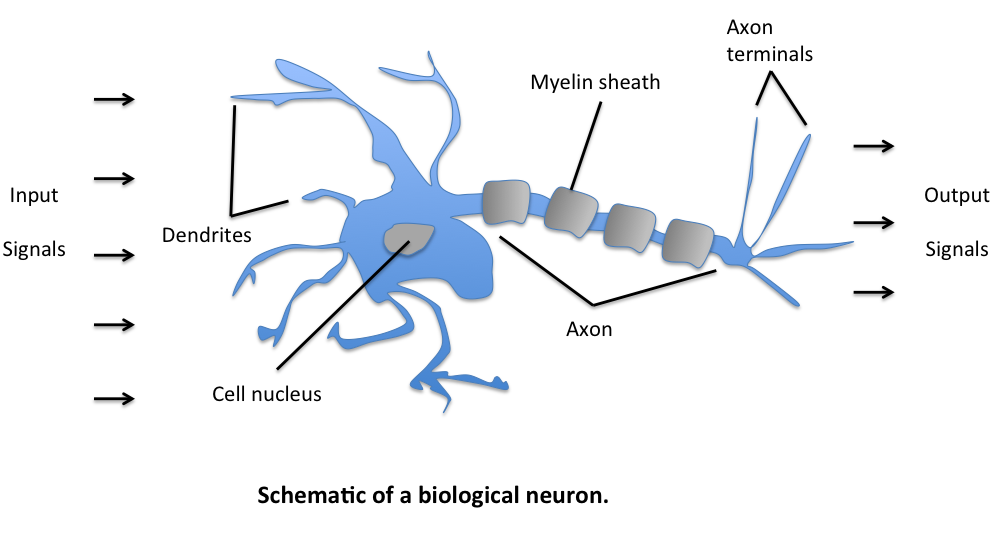
\includegraphics[width=10cm]{perceptron_neuron.png}
\centering
\caption{A biological neuron \cite{neuron}.} 
\label{fig:biologicalneuron}
\end{figure}

The artificial neuron has four main components: inputs $x$, weights $w$, the activation function $f(x)$ and the output. The inputs are the features or attributes, also known as feature vector, which is simply represented as an n-dimensional vector consisting of binary or numerical values. These inputs are the equivalent of the input signals being received by the dendrites in Figure \ref{fig:biologicalneuron}. These inputs are then multiplied by weights and fed into an activation function. The output is the result of this activation function. In its simplest form, the output of an activation function is binary, which in the biological neuron translates to whether the neuron is firing an electrical signal or not. There are many types of activation functions, however the popular ones are the sigmoid function, $tanh$ function, and the softmax function. If an activation function does not output a discrete value, then a threshold is set, for example:  \[ f(x) =
  \begin{cases}
    1       & \quad \text{if } x \geq 0\\
    0       & \quad \text{if } x < 0
  \end{cases}
\]
Training a model involves determining the right weight values that causes the artificial neuron to output the correct result. This is done using gradient descent on the training set. 

\begin{figure}[h]
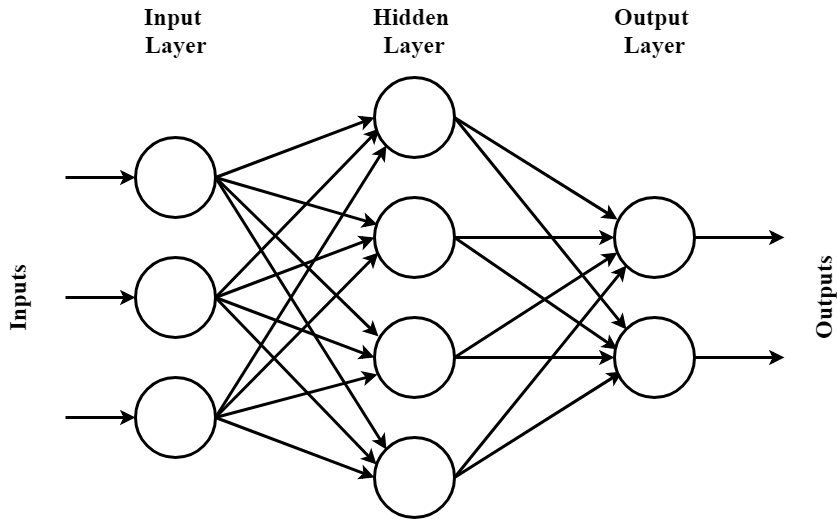
\includegraphics[width=10cm]{feedforward.png}
\centering
\caption{A feed forward network.} 
\label{fig:feedforward}
\end{figure}

\subsection{Feed Forward Neural Network}
A feed forward neural network is an architecture that consists of layers of neurons, where the output of one neuron can be fed into another neuron, without any loops \cite{jain1996artificial}. Therefore, all information that is fed into the input layer flows through the hidden layers until it reaches the output layers, such that the outputs of each layer only effects the next layer, without any feedback \cite{jhaartificial}. An example of a feed forward network can be seen in Figure \ref{fig:feedforward}, which contains an input layer, one hidden layer, and an output layer. If a feed forward network has more than one hidden layer, then it is called a deep architecture. 

Some of the architectural decisions that must be taken with feed forward networks is deciding how many hidden layers and nodes should be included in the network. Cybenko \cite{cybenko1989approximation} introduced the first version of the universal approximation theorem which states that a feed-forward network with one hidden layer and a finite number of neurons can learn most problems when given the appropriate parameters. Hornik \cite{hornik1991approximation} further expands on this theorem and shows that it is not the choice of activation function, but rather the choice of feed forward architecture that brings out the full potential of being universal approximators. Given this theorem, one might wonder why anyone would need a deep architecture. While this theorem holds for \textit{representing} a wide array of problems, it does not deal with the algorithmic \textit{learnability} of parameters. It was always possible to build deep networks with feed forward networks. They were just not particularly good at training them before Hinton et al. \cite{hinton2006fast} showed how a many-layered feed forward neural network can be effectively trained one layer at a time. 

\section{Financial Forecasting}
Stock market prediction is one of the most challenging areas of research lately due to stock markets being essentially dynamic, non-linear, complicated, non-parametric and chaotic in nature \cite{tan2005brain}. Additionally, stock market movements are influenced by several macroeconomical factors such as political events, economic conditions, movement of other stock markets and investor expectations \cite{zhang2009stock}. Despite these challenges, predicting stock markets is a very attractive problem to solve thanks to the high benefits that it can offer through many commercial applications \cite{majhi2007stock}. 

The difficulty of stock market prediction has raised questions on whether this is achievable. The EMH and the Random-Walk Hypothesis both claim that there is no value to predicting a market price since the current price truly reflects the value of the stock. However, researchers believe that markets are inefficient, partly due to psychological factors of the various market participants, along with the inability of the markets to immediately respond to newly released information \cite{jensen1978some}. 

The recent trend is to develop models for forecasting financial data \cite{majhi2007stock}. Forecasting models can either be statistical or soft-computing models. The most popular statistical forecasting model is the Auto-regressive Integrated Moving Average (ARIMA) model. It predicts future values of a series based on its own inertia and is suitable for short-term forecasting with data that contains stable or consistent patterns. ARIMA however is a linear non-stationary model, therefore other alternatives must be considered for forecasting non-linear series, such as stocks \cite{wang1996stock}. 

\subsection{Soft Computing Techniques}
Unlike statistical models, AI models such as ANNs, fuzzy systems, and genetic algorithms are driven by multivariate data with no required assumptions, and thus have been applied to forecast financial variables on several occasions \cite{zhong2017forecasting}. 

\subsection{Equation Discovery}
Equation discovery is a machine learning approach for learning quantitative laws and models from measured numeric data, expressed in the form of equations \cite{Todorovski2010}. Equation discovery can also be used for financial forecasting.  \cite{kazakov2008equation}  used LAGRAMGE, an equation discovery tool, for modelling macroeconomic variables. There are an infinite amount of equations that can be found when trying to model a situation. To help restrict the search space, LAGRAMGE makes use of user defined context free grammars. Georgiev and Kazakov in \cite{Georgiev2012Equation} used LAGRAMGE to search for ordinary differential equation models for macroeconomic data. They conclude that differential equations match ordinary ones with regards to accuracy, while having a better forecast range \cite{Kokov2012Equation}.  

\subsection{Artificial Neural Networks}
One popular technique for financial forecasting is to use ANN based models, which are capable of approximating any nonlinear function to a high degree of accuracy. They are less sensitive to error term assumptions and can tolerate noise and chaotic components \cite{majhi2007stock}. ANNs have been used for stock market prediction for decades. in 1990, Kamijo and Tanigawa \cite{kamijo1990stock} used recurrent neural networks (RNN) while Ahmadi \cite{ahmadi1990testability} used back propagation (BP) neural networks to predict the stock market. Trippi et al. \cite{trippi1992trading} introduced a neural-network based intraday trading system for the S\&P 500. 

Despite being suitable for financial time series forecasting, Lawrence et al. \cite{lawrence1998noisy} point out that excessive noise in data when training BP networks could resort to the network taking a naive solution, such as predicting the most common output. Furthermore, achieving the desirable result requires a careful selection of a combination of network parameters, such as learning rate, number of hidden layers and number of nodes in each layer \cite{hussain2008financial}. It has been shown that designing an ANN with the least complex architecture and the right input variables can greatly improve efficiency and accuracy \cite{atsalakis2009surveying}. Therefore, when it comes to using ANNs for financial forecasting, it is essential to choose the most influential and representative inputs which, as mentioned earlier, can be any of the various macroeconomic factors that affect the stock market \cite{zhong2017forecasting}. 

\subsection{Hybrid Algorithms and Ensemble Learning}
Nowadays prediction performance is being improved by hybridising several AI techniques. Tsaih et al. \cite{tsaih1998forecasting} integrated the rule-based technique and ANNs to predict daily S\&P500 direction changes on a daily basis. Zhang et al. \cite{zhang2009stock} predicted short term and long term stocks using a BP neural network incorporated with an improved bacterial chemotasix optimisation (IBCO). Asadi et. all \cite{asadi2012hybridization} proposed a combination of data preprocessing methods, genetic algorithms and Levenberg-Marquardt (LM) algorithm for learning feed forward neural networks. Through data transformation and input selection pre-processing methods, the resulting model yielded good prediction results and coped well with stock market fluctuations. In 2009, Ou and Wang \cite{ou2009prediction} used ten data mining techniques to predict the Hang Seng index. These include Linear Discriminant Analysis (LDA), Quadratic Discrimant Analysis (QDA), K-nerarest neigbour classification, Tree based classificatio, ANNs, Support Vector Machines and Least Squares Support Vector Machine (LS-SVM). For their experiment, SVM and LS-SVM had the best predictive performance. In 2010, Hadvandi et al. \cite{hadavandi2010developing} used a combination of genetic algorithms and feed forward neural networks to predict the TEPIX stock index.

Another recent trend in financial time series prediction is the use of ensemble learning. Ensemble learning is the combination of predictions from individually trained classifiers to form a single predictive model. Research has shown that an ensemble is often more accurate than any of the individual classifiers in the ensemble \cite{opitz1999popular}. Apart from improving the prediction performance, ensemble techniques can be used for model selection. Bagging \cite{breiman1996bagging} is one example, where classifiers train on several sub samples of the training data and then, by majority voting, the most-voted class is predicted. Another ensemble technique is random subspace, which randomly selects some features from the given feature space. A model will be built on each subspace, and finally integrated by majority vote, similar to bagging. 

\chapter{Problem Analysis}
\section{Stock Market Forecasting}
The previous chapter mentioned several techniques for stock market prediction such as using statistical models, ANNs, SVM and ensemble methods. Despite having all these different approaches, the no free lunch theorem \cite{wolpert1997no} states that there is no singular model that works best for every problem. This means that while a particular approach might work for a particular problem, it might not hold for another. 

Atsalakis and Valavanis \cite{atsalakis2009surveying} provide an excellent survey on 100 scientific articles on stock market forecasting. These articles together model 24 stock market indices from around the world, both from well developed markets such as the U.K., U.S.A and Japan, and emerging markets such as Latvia, Singapore and Turkey. The most popular region for research are American stock indices such as S\&P 500, NASDAQ and Dow Jones.

\subsection{Inputs}
As mentioned earlier,  it is essential to choose the most influential and representative inputs when it comes to financial forecasting \cite{zhong2017forecasting}. In the aforementioned survey \cite{atsalakis2009surveying}, the number of inputs used ranged from 2 to 61 variables. 

The most commonly used inputs are stock index data, which can either be opening or closing prices, as well as daily highest and lowest values. This suggests that a significant amount of research prefer to use simple input data to provide predictions. \cite{barnes2000study, donaldson1999neural, halliday2004equity, tan1995conservative, pai2005hybrid, pantazopoulos1998financial} all used daily closing prices as input, while \cite{andreou2000testing, fernandez2000profitability, pan2005predicting,tang2002web} also used the closing price from previous days. 

Some studies have combined closing prices with other stock market indices, or external factors such as macroeconomical and financial variables. Examples of external factors are currency exchange rates, gold coin value, interest rates and earning announcements. \cite{ajith2003hybrid} attempts to predict the NASDAQ stock index by using closing prices from NASDAQ and 7 other indices. \cite{huang2005forecasting} uses both the S\&P 500 and USD/YEN exchange rate to predict the NIKKEI stock market index. \cite{phua2001neural} forecasts the Singapore stock exchange using volume, opening, lowest, highest and closing index prices of the DJIA, NASDAQ, HIS and NIKKEI indices. \cite{siekmann1999information} used the DJIA index and the USD/EURO exchange rate to predict the DAX stock market index. \cite{tabrizi2000stock} forecasts the TEPIX stock index using the gold coin value and the USD exchange rate. \cite{levodeanschi2016} investigated the impact of using earnings calendar information in portfolio construction techniques. In general, \cite{atsalakis2009surveying} highlights that researchers tend to use a combination of exchange rates and stock index values for predicting emerging markets as they are more likely to be influenced by these factors than well established markets. Other papers that used macroeconomical and financial factors are: \cite{gradojevic2002neuro}, which used lagged interest rates and lagged order flow; \cite{thawornwong2004adaptive}, which used thirty one financial and economic variables including producer price index, industrial price index, consumer price index and money stock; and \cite{setnes1999fuzzy}, which predicted the Amsterdam stock exchange (AEX) using Dutch macroeconomic data such as money supply, long and short term interest rates, economic growth and inflation. 

Almost all the articles mentioned in \cite{atsalakis2009surveying} found input data preprocessing to be useful and necessary. Sensitivity analysis is sometimes employed to help remove any redundant inputs. In several cases, input data has a wide range of values, which might reduce the effectiveness of training procedures. This can be solved by normalising the data. Alternative techniques are to use Principal Component Analysis (PCA) \cite{ajith2003hybrid}, Z-score \cite{leigh2002analysis}, and an ANFIS techniques used by \cite{atsalakis2006neuro}. 

\subsection{Forecasting Methodologies}
Neural network architectures such as feed forward and recurrent networks are the most popular forecasting architecture, amounting to 60\% of the articles surveyed in  \cite{atsalakis2009surveying}. \cite{ajith2003hybrid, andreou2000testing, pantazopoulos1998financial,phua2001neural, refenes1997neural, thawornwong2004adaptive} used feed forward neural networks while \cite{barnes2000study, leigh2002analysis, witkowska1995neural} used back propagation neural networks. Architectures typically span between one or two hidden layers, while the maximum number of input nodes used is 52. \cite{atsalakis2009surveying} comments that despite neural networks are suitable for market forecasting, difficulties tend to arise when defining the anatomy of the model, and so far the best way to determine the optimal architecture is through trial and error. 

\section{Data} 
\label{sec:data}
This work requires both macro-economic data and stock market index data. The following subsections describe the data that has been collected. The following chapter will then explain how this data was transformed and manipulated.

\subsection{Macroeconomic Data}
Since this work predicts the direction of the UK stock market, it made sense to focus on collecting macro-economic data for the UK. To simplify the model, the scope of learning had been reduced to five macro-economic variables: Inflation Rate, Interest Rate, Balance of Trade, Unemployment Rate and GDP. These parameters were chosen because they are commonly used in literature, both for stock market prediction and modelling of macroeconomic variables. A definition for these terms can be found in section 2.1. This data is provided by the UK Office for National Statistics. They provide yearly, quarterly and monthly data for inflation and unemployment rate, yearly and quarterly data for GDP and balance of trade, and daily data for interest rate. 

\subsection{Stock Market Index Data}
This work requires historical closing prices from some of the top global financial stock market indices. Apart from FTSE, which is what will be predicted, data had to be collected for the following stock market indices: STOXX 50, S\&P 500, Nikkei 225, DAX 30, CAC 50 and Hang Seng. These indices where chosen precisely because they represent the most influential economies in the world, and are often used in literature for financial forecasting. Stock market indices from emerging markets are less likely to influence well established markets such as the UK.  More information about these stock market indices can be found in Table \ref{tab:indices}. All these stock market indices where collected from Yahoo Finance, except for FTSE, which was collected from \textit{www.investing.com}. 

\section{Objectives}
\label{sec:objectives}
This work seeks to measure the impact of external factors, particularly the closing prices of other stock markets and macroeconomical data, when predicting the direction of the FTSE stock market index. It does not seek to introduce a new trading tool that maximises profit, or a state-of-the-art architecture for financial forecasting, but rather investigate how particular data sets can improve predictive performance. Overall, this work seeks to confirm the following null hypotheses:

\begin{enumerate}
    \item \label{h1} \textbf{The use of macroeconomic parameters improves the performance for predicting the direction of a stock market index.}
    \item \label{h2} \textbf{The use of closing prices from other stock market indices improves the performance for predicting the direction of a stock market index.}
    \item \label{h3} \textbf{If both previous hypotheses are true, then the combination of macroeconomic parameters and closing prices from other stock market indices will further improve the performance for predicting the direction of a stock market index.}
\end{enumerate}

\section{Requirements}
\label{sec:requirements}
The requirements for this work are:

\begin{enumerate}
    \item \label{basecase} \textbf{Formulate a base case for predicting the direction of the FTSE index:} This base case will be a simple model that only uses historical prices of the FTSE index, and not use closing prices from other stock indices or macroeconomical parameters. The performance of other methodologies will be compared with this base case to determine whether an improvement in predictive performance has been made.  
    \item \textbf{Formulate a model that incorporates historical FTSE closing prices with macroeconomical parameters for predicting the direction of the FTSE index:} This model will be used to confirm whether hyptothesis \ref{h1} holds.
    \item \textbf{Formulate a model that incorporates historical FTSE closing prices with closing prices from other stock market indices for predicting the direction of the FTSE index:} This model will be used to confirm whether hypothesis \ref{h2} holds.
    \item \textbf{Formulate a model that incorporates historical FTSE closing prices with both macroeconomical parameters and closing prices from other stock market indices for predicting the direction of the FTSE index:} This model will be used to confirm whether hypothesis \ref{h3} holds.
    \item \label{framework} \textbf{Develop a framework that can be used to train, predict and evaluate the performance of the above models:} More information on the performance measures and evaluation criteria will be covered in the next section. 
\end{enumerate}

\section{Performance Measures and Evaluation Criteria}
Performance measures can be classified as statistical measures or non-statistical measures \cite{atsalakis2009surveying}.

Examples of statistical measures are the root mean square error (RMSE), the mean absolute error (MAE), the mean squared prediction error (MSPE), $R^2$, F1 score and statistical indicators such as autocorrelation, correlation coefficient, and standard deviation. 

Non-statistical performance measure are less common, and in financial forecasting are typically related with the economical side of the forecast. An example is the hit rate, which measures the percentage of correct predictions of the model. Other non-statistical measures deal with the profitability of the model, such as annual rate of return and average annual profit.

This work involves predicting the direction of the FTSE stock market index, thus making it a binary classification problem. As mentioned in the previous section, it is pertinent to understand that the aim of this work is to determine whether combining particular sets of data will improve the predictive performance of an algorithm, and not to find the a state-of-the-art approach for maximising profits. Nonetheless, prediction accuracy does not directly equate to more profit. When predicting direction of stock markets, you could achieve a high accuracy, however one incorrect prediction could be a drop large enough to wipe out any profits made in previous prediction. Thus, these findings are not intended to be used directly in complete trading strategies, despite perhaps being a stepping stone to improving trading strategies in the future. 

Since we have a binary classification problem, is does not make sense to use statistical performance measure such as RMSE, MAE and $R^2$ as they require continuous values. They would have been suitable to use if this work involved predicting a continuous value such as the closing price, or the percentage increase. The two measures that will be performed in this work will be \textbf{accuracy} and \textbf{F1 score.} 

Both the accuracy and F1 score require the following items to be counted:

\begin{enumerate}
    \item \textbf{True Positives (TP)}: This is when a result correctly predicts that the index will rise (the positive condition).
    \item \textbf{True Negatives (TN)}: This is when a result correctly predicts that the index will fall (the negative condition).
    \item \textbf{False Positives (FP)}: This is when a result predicts incorrectly that the index will rise, when it actually falls.
    \item \textbf{False Negatives (FN)}: This is when a result predicts incorrectly that the index will fall, when it actually rises.
\end{enumerate}

Figure \ref{fig:tptnfpfn} helps visualise what these terms mean.

\begin{figure}[h]
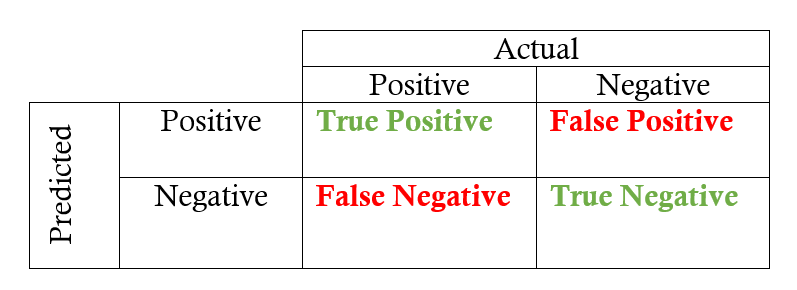
\includegraphics[width=10cm]{tptnfpfn.png}
\centering
\caption{Matrix of terminology for true and false negatives and positives \cite{precisionandrecall}} 
\label{fig:tptnfpfn}
\end{figure}

The accuracy can be calculated as follows: 
\begin{equation}
\label{eq:accuracy}
accuracy=\frac{TP + TN}{TP + TN + FP + FN}
\end{equation}
This is simply the summation of correctly predicted values divided by the total number of data items.

Having accuracy as the sole performance metric is not good enough. As an example, imagine a model that identifies whether people at an airport are terrorists or not. This model can reach over 99\% accuracy simply by labelling all passengers as not a terrorist, because typically there are only a handful of terrorists compared to the millions of passengers that travel in airports every year. The real performance metric in this case would be measuring how well it identifies terrorists, therefore true positives. The metric we are after is known as \textbf{recall} in statistics. Recall is the measure of the model's ability to find all relative cases (true positives) within a dataset. It can be measured by the following formula:

\begin{equation}
recall=\frac{TP}{TP + FN}
\end{equation}

Recall is also referred to as true positive rate, probability of detection and sensitivity.  

Another important statistical metric is \textbf{precision}, which measures the ability of a model to identify only the relevant data points. If we relied of just recall, then labelling all the results as positive would result in a perfect recall score of 1. Such a model would however suffer from low precision. Precision is calculated as:

\begin{equation}
precision=\frac{TP}{TP + FP}
\end{equation}

Precision is also referred to as the positive predictive value. 

Depending on the problem at hand, statisticians would prefer to maximise either recall or precision at the expense of the other. As an example, in cancer screening models, one would rather maximise recall, therefore identifying patients with cancer, while accepting lower precision. However in certain cases, such as stock market prediction, a good balance of precision and recall would be appreciated, because predicting incorrectly whether a stock will increase or decrease will both have the same severe consequences: profit loss.

The ideal metric for this particular problem, stock market prediction, is the F1 score, which is a metric that combines both precision and recall. The F1 score can be calculated as:

\begin{equation}
\label{eq:f1}
F_1=2 \times \frac{precision \times recall}{precision + recall}
\end{equation}


\section{Discussion}
\label{sec:discussion}
This chapter began by comparing and contrasting past financial forecasting techniques, primarily on what data has been modelled, how it was preprocessed, and what architectures were used. It was also shown that stock market index prediction is sometimes combined with other external data, such as economical data, to help improve prediction performance. Other works also took into consideration the closing prices of other stock market indices. However, to our knowledge, there seems to be a gap in literature where both macroeconomic data and the closing prices of other markets are used to predict a stock market index. 

Both an ensemble approach consisting of a two staged approach and feed forward networks will be introduced in the next chapter that will conform to the requirements in Section \ref{sec:requirements}. As previously mentioned, ensemble methods have been shown to improve prediction performance over individual classifiers in the ensemble \cite{opitz1999popular}. Both stages of the ensemble will use a feed forward artificial neural network. the ensemble approach will only be used for adding macroeconomic data, while simple feed forward networks will be used for the rest of the models. The main reason for using an ensemble approach when incorporating macroeconomic data was due to difference in statistical properties between the stock market data and macroeconomic data. Stock market data consists of data that fluctuates daily, while macroeconomic data is either quarterly, monthly or daily and in some cases, such as interest or inflation rate, remains constant from time to time. The macroeconomic data in the ensemble method will be used as a tool for model selection of different stock market predictors. More details about the ensemble method will be explained in the following chapter.  

The motivation for using feed forward networks was due to their popularity as a choice of architecture for several financial forecasting applications. Nonetheless, the main aim of this work is not to determine the best architecture for financial forecasting, but to investigate whether different sets of data can help improve performance. From the literature review performed in this work, feed forward networks seemed to be a safe and easy choice. They do not necessarily require a complex architecture to achieve good performance, they can work well even with small amounts of data (therefore efficient), and they are well established architectures for financial forecasting.    

This work involves predicting the direction of the FTSE stock market index. A slightly different approach from other works will be taken when factoring in the closing price of other stock market indexes. The approach presented in this work will follow the sun and take into consideration the closing prices of Asian stock market indices that have closed on the same day that we are trying to predict. Taking a look at the opening and closing times of stock markets in table \ref{tab:markets}, both the Hong Kong and Tokyo stock exchange close before the London stock exchange has opened. For other stock market indices and the FTSE index itself, it shall consider the closing prices starting from the previous day.       

\chapter{Design and Implementation}
\section{Tools}
As discussed in Section \ref{sec:discussion}, the most suitable approach to confirm the hypotheses mentioned in Section \ref{sec:objectives} was to utilise machine learning techniques, particularly feed forward networks and ensemble learning. A decision had to made on what programming language and libraries to use. Java, R, Matlab and Python were considered for this work. As for machine learning libraries, Weka, TensorFlow, Theano, DL4J (Deep learning for Java) and other packages and functionality baked into Matlab and R were taken into consideration. Tghe final decision was to use TensorFlow with Python, primarily due to the popularity of TensorFlow in the industry and research community. 

TensorFlow is an open source software library for high performance numerical computation, but is widely used for machine learning applications, such as neural networks. It was developed by the Google Brain team, hence it is heavily used by Google itself in its own applications. Despite having only been released in 2015, it has already established itself as one of the most popular libraries in the industry. The excellent documentation, the ease of deploying across different platforms such as CPUs and GPUs, the endless use cases that TensorFlow can be applied to, the good readability and high level of abstraction are some of the reasons why TensorFlow rose to fame so quickly. Compared to other libraries, such as Theano, it requires less functionality hacking for tailoring to specific problems, hence allowing developers to apply and try different architectures and parameters quickly and effectively. As a result, TensorFlow has developed a vibrant community around it, which means that it will continue to be maintained and improved for years to come. These reasons ultimately made TensorFlow the library of choice for this work.         

TensorFlow was specifically built to run with Python, but also offers APIs for Java, C and Go. However, these APIs are not as extensive as the Python API. Naturally, Python was chosen for this work. Python is a dynamically typed language that supports several programming paradigms such as object-oriented, imperative and functional paradigms. It also serves as a great scripting language, making it suitable for quick and easy experimentation. It is free and open source, unlike Matlab, and is available on several operating systems. The version of Python used in this work was version 3.6.5, while version 1.8.0 of TensorFlow was used.

\section{Data Preprocessing}
Section \ref{sec:data} gave an overview of what data was required for this work, how it was obtained, and what the data consists of. Just like for any times series analysis and machine learning problem, data must be made stationary in order to remove trend and seasonality. An exercise was carried out to determine the optimal way to make the data stationary. Data was tested for stationarity by applying the Augmented Dickey-Fuller (ADF) test. The ADF test is a type of statistical test called a unit root test. A unit root test determines how strongly a time series is defined by a trend. The result is interpreted using the p-value from the test. A p-value below a certain threshold, typically 5\%, suggests that a series is stationary, otherwise it is described as non-stationary. 

Section \ref{subsec:stationary} mentioned several ways to make data stationary. Through trial and error, the chosen approach for making this data stationary was:
\begin{align}
n_i = \frac{x_i}{\max(x)} \label{eq:normalised} \\ 
y_i = \log_e\frac{n_i}{n_{i-1}} \label{eq:log} 
\end{align}

Where $x$ is the dataset, $x_i$ the value of $x$ at index $i$, $n_i$ is the normalised value at index $i$, and $y_i$ the stationary value at index $i$. 

This approach is also convenient for extracting the expected outputs, hence the direction of the index for a particular day. These expected outputs are essential for both training and testing models. A value of 1 signifies that an index will rise, while a value of 0 signifies that an index will fall. In its nature, the natural logarithm of 1 results in a value of 0. In Equation \ref{eq:log}, a logarithmic of 1 can only be achieved if the index value did not change from one day to another. If the value of the index did rise, then the natural logarithmic of a value greater than 1 would be positive, otherwise negative. Therefore, whether $y_i$ is positive or negative translates to stock index either rising or falling.

The last step in preparing the data was to split the data into training and testing data. The chosen approached was to take 80\% of the data for training, and 20\% for testing.

\section{Finding the Optimal Parameters}
When working with feed forward networks, achieving an optimal result requires a careful selection of a combination of network parameters, such as learning rate, number of hidden layers and number of nodes in each layer \cite{hussain2008financial}. Since the aim of this work is not to find a state-of-the-art architecture, but rather measure the impact of different data sets of data on financial forecasting, it was decided to keep the architecture simple with just one hidden layer. Other than being less complex and computation heavy, literature suggests that a feed forward network with one hidden layer can learn most problems when given appropriate parameters \cite{cybenko1989approximation}. Nonetheless, a methodology for finding the best parameters had to be formulated for each model so as to have a fair comparison for predictive performance.   

Despite the models in this work having different architectures and inputs, the approach for finding the the optimal parameters followed the same pattern. Each model was run several times while iterating through different combinations of learning rates and number of hidden nodes. The range of parameters was mainly chosen through trial and error. Each run consists of both training and testing. Performance metrics \ref{eq:accuracy} and \ref{eq:f1} were recorded after each run. A common practice in neural networks is to initialise the network with random weights. Consequently, this means that such a model is not pure, therefore it will not give the same result when given the exact same parameters and inputs. To overcome this, each model was run a further 20 times for ever combination of parameters, and the average F1 score and accuracy were recorded. These performance metrics were then plotted in a 3D graph of number of nodes vs learning rate vs accuracy or f1. This graph helped visualise the impact of the chosen parameters and thus made it possible to choose the optimal combination of parameters. In the case that the peak performance was recorded on the edge of the graph, the same exercise would be repeated with different ranges of learning rates and number of hidden nodes around that peak.

As one can imagine, such an exercise takes a long time to run. For example, iterating through 10 different learning rates and 10 different number of hidden nodes, while taking the average of 20 individual runs for each parameter combination would mean that the model will be executed 2000 times. Optimising the code for parallelism was helpful. Thankfully, Tensorflow automatically performs computations on a graphics card when it detects an Nvidia GPU installed, naturally giving a speed boost to computation speed. 

\section{The Base Case}
\section{Hypothesis 1: Incorporating Other Stock Market Indices}
\section{Hypothesis 2: Incorporating Macroeconomical Parameters}
\section{Hypothesis 3: Incorporating Macroeconomical Parameters and Other Stock Market Indices}


\chapter{Results and Evaluation}

\chapter{Conclusions}
\printbibliography
\end{document}